\documentclass[11pt,solution]{cpgedev}

\cpgegeometry{tablet} 
\cpgetheme[logo=rabat]{ibnghazi}
%\cpgeconfig{mines}
\cpgefont{libertine}

\usepackage[hypcap=false]{caption}
\usepackage{parskip} 

 
\Matiere{Mathématique}
\Document{Sujet de concours} 
\Concours{Mines et Ponts} 
\Epreuve{Mathématiques 2}
\Session{2024} 
\Duree{4} 
\Auteur{Sadik Boujaida}  
\Classe{MP}
\Preauteur{Corrigé proposé par}
\Email{ibouja@gmail.com}
\Website{https://github.com/texbouja/Mines2024}

\cpgesetuplists{%
    enumi=  {n=Q|1|, m+ ,s=12pt},
    enumii= {n=|Q|.|a|},
    enumiii={n=|Q|.|q|.|i|}
}

\cpgesetlabel{parti}{Partie |I|}
\cpgesetlabel{partii}{Section |A|}

\cpgesetupmath{symbol={corps=R}}
\let\i\isymb
\def\X#1{X_{\{#1\}}}

\begin{document}  

\cpgesethead
    (|concours| -- |session| -- |epreuve|) 
    ()
    (|problem|)
\cpgesetfoot()(|pages|)()

\cpgesettitle{
    \ifdefmeta{document}
        |document| \par \bigskip\bigskip 
    \fi
    \ifdefmeta{concours}
        |concours| \\
    \fi
    \ifdefmeta{epreuve}
        |epreuve|   \\
    \fi
    \ifdefmeta{session}
        |session|  \\
    \fi 
    \ifdefmeta{auteur}
        \ifsolution
            \par \bigskip
            |auteur| 
        \fi
    \fi
}
\cpgesettitle*{
        |document| 
    \bigskip\hrule\bigskip\bigskip
        |concours|
        |epreuve| 
        |session|  \vskip 1cm plus .2fill 
    \ifsolution 
        |auteur| 
        |website|  
    \fi
}

\titre
%\devoir\op{name =ds,number=11,after title=|duree|}{Devoir surveillé}(Théorie des graphe)
\begin{enonce}{mines24m2}\op{score}
    [](Phénomènes de seuil dans les graphes)
    <enonce>
    \everymath{\displaystyle}
    Dans ce problème, $n$ désigne un entier supérieur à 1 .
    On désigne par $\iic{1,n}$ l'ensemble des entiers compris entre 1 et $n$. 
    
    Le groupe symétrique des permutations de $\iic{ 1, n }$ est noté $\mathcal{S}_n$. 
    
    L'ensemble des matrices carrées d'ordre $n$ à coefficients réels est noté $\mathcal{M}_n(\mathbf{R})$. 


    Le cardinal d'un ensemble fini $E$ sera noté $\operatorname{card}(E)$ ou $|E|$. 

    Un graphe $G$ est un couple $(S, A)$ où :

    \xit\i+
        $S$ désigne un ensemble fini non vide d'éléments appelés sommets du graphe $G$ 
    \xit
        $A$ désigne un ensemble éventuellement vide d'éléments appelés arêtes du graphe $G$, une arête étant un ensemble $\left\{s, s^{\prime}\right\}$ où $s$ et $s^{\prime}$ sont des sommets distincts de $S$.
    \exit

    Un sommet n'appartenant à aucune arête est dit isolé.
    Par convention, le graphe vide est le couple d'ensembles vides $(\varnothing, \varnothing)$.

    On peut représenter un graphe non vide dans un plan à l'aide :
    \xit\i+ 
        de disques schématisant les sommets du graphe
    \xit
        de segments reliant ces disques pour les arêtes du graphe.
    \exit 
    Par exemple, on a représenté sur la \textsc{Figure 1}, le graphe $G=(S, A)$ avec~:
    \<
        S=\iic{ 1,9 } \text { et } 
        A=\delim\sz1\{\{1,2\},\{1,5\},\{1,6\},\{2,3\},\{2,9\},\{2,8\}\}
    \>
    \begin{center}
        \ifdark 
            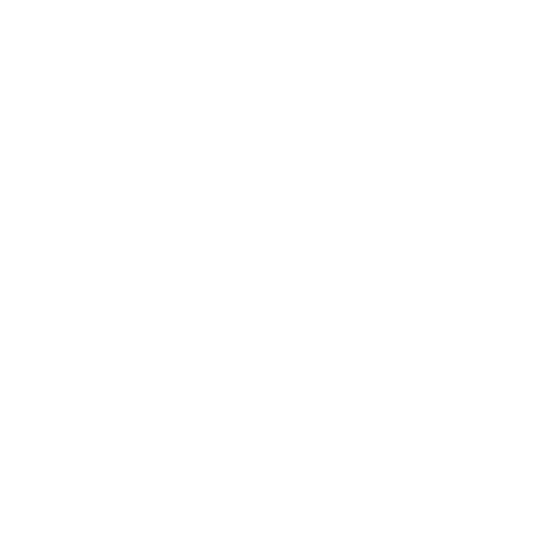
\includegraphics[width=4.5cm]{graphs/graph-dark-0}
        \else 
            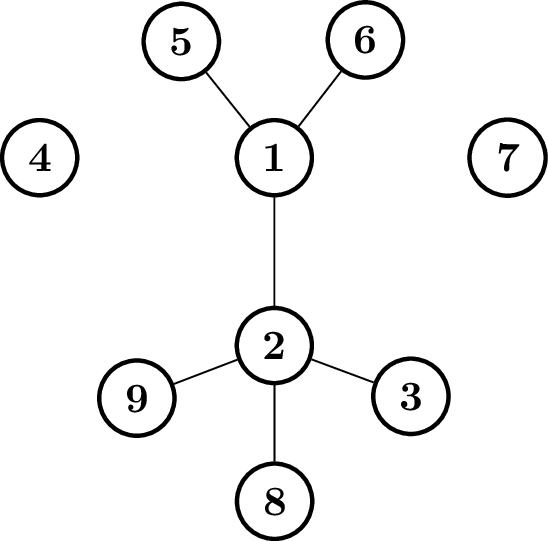
\includegraphics[width=4.5cm]{graphs/graph-0}
        \fi 
        \captionof{figure}{un graphe à 9 sommets et 6 arêtes}
    \end{center}



    On remarquera que les arêtes sont constituées de deux sommets distincts, ce qui interdit la présence de "boucles" reliant un sommet à lui-même.
    
    De plus, une même arête ne peut être présente plusieurs fois dans un graphe.



Un type de graphe utilisé dans ce problème est l'étoile.

Une \textbf{étoile} de \textbf{centre} $s$ et à $d$ \textbf{branches} avec $d$ entier naturel non nul, est un graphe $(S, A)$ où $S=\left\{s, s_1, s_2, \ldots, s_d\right\}$ est de cardinal $d+1$, et $A$ est du type
\<
A=\left\{\left\{s, s_1\right\},\left\{s, s_2\right\}, \ldots,\left\{s, s_d\right\}\right\}
\>

On a représenté \textsc{Figure 2} une étoile de centre 4 à 5 branches avec $S=\{1,3,4,5,6,8\}$.

\begin{center}
    \ifdark 
        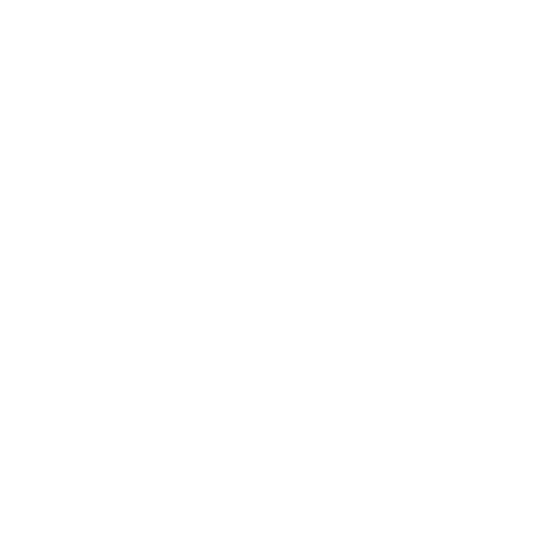
\includegraphics[width=4.5cm]{graphs/graph-dark-1}
    \else 
        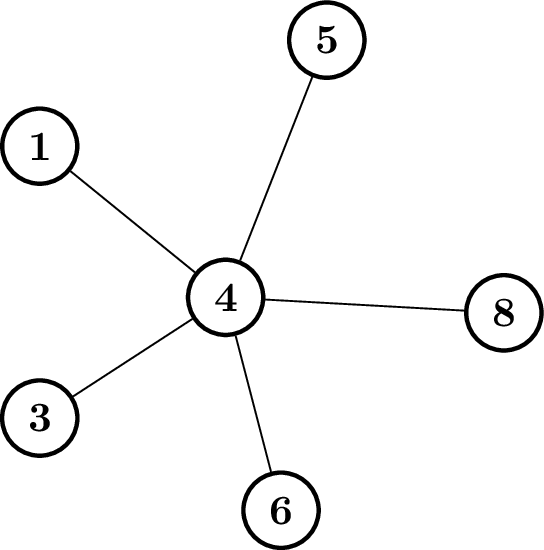
\includegraphics[width=4.5cm]{graphs/graph-1}
    \fi 
    \captionof{figure}{une étoile à 5 branches}
\end{center}

%FIGURE 2 - une étoile à 5 branches

Soient $G=(S, A)$ et $G^{\prime}=\left(S^{\prime}, A^{\prime}\right)$ deux graphes ; on dit que :
\xit\i+ $G^{\prime}$ est inclus dans $G$ si $S^{\prime} \subset S$ et $A^{\prime} \subset A$
\xit $G^{\prime}$ est une copie de $G$ s'il existe une bijection $\sigma$ de $S^{\prime}$ dans $S$ telle que :
\exit 

\<
\forall\left(s^{\prime}, t^{\prime}\right) \in S^{\prime} \times S^{\prime} \quad\left\{s^{\prime}, t^{\prime}\right\} \in A^{\prime} \Longleftrightarrow\left\{\sigma\left(s^{\prime}\right), \sigma\left(t^{\prime}\right)\right\} \in A
\>

Par exemple, le graphe de la Figure 1 contient plusieurs copies d'étoiles à une branche (correspondant aux segments), plusieurs copies d'étoiles à deux branches, mais aussi une copie d'une étoile à 3 branches (de centre 1) et une copie d'une étoile à 4 branches (de centre 2).

Dans une première partie, on étudie quelques propriétés algébriques des matrices d'adjacence. 

On introduit ensuite la notion de fonction de seuil en probabilité des graphes aléatoires. Les deux parties qui suivent la première partie sont indépendantes de celle-ci, et sont consacrées à l'étude de deux exemples.

\partie\w
    (Quelques propriétés algébriques des matrices d'adjacence)
    <parti1>

Soit $G=(S, A)$ un graphe non vide où $|S|=n$. Indexer arbitrairement les sommets de 1 à $n$ revient à choisir une bijection (appelée aussi indexation) $\sigma$ entre $\iic{ 1, n }$ et $S$. On pourra alors noter :
\<
S=\{\sigma(1), \sigma(2), \ldots, \sigma(n)\}
\>
où $\sigma(i)$ est le sommet d'index $i$.
Une indexation $\sigma$ étant choisie, on définit la matrice d'adjacence $M_{G, \sigma}$ du graphe $G$ associée à $\sigma$ comme étant la matrice de $\mathcal{M}_n(\mathbf{R})$ dont le coefficient situé sur la $i^e$ ligne et la $j^e$ colonne est :
\<
\left(M_{G, \sigma}\right)_{i, j}= \begin{cases}1 & \text { si }\{\sigma(i), \sigma(j)\} \in A \\ 0 & \text { sinon }\end{cases}
\>


On remarquera d'une part que la matrice $M_{G, \sigma}$ est toujours symétrique (car pour tous $i$ et $j$ entiers, $\{i, j\}=\{j, i\}$ ) et d'autre part que les termes de la diagonale sont tous nuls (pas de boucle dans un graphe).

Voici par exemple la matrice d'adjacence $M_{G, \text { ld }}$ du graphe $G$ représenté sur la \textsc{figure~1}~:
\<%\def\arraystretch{.5}
    M_{G,\id}=\xmatrix\s(
        0&1&0&0&1&1&0&0&0 \\ 
        1&0&1&0&0&0&0&1&1 \\
        0&1&0&0&0&0&0&0&0 \\
        0&0&0&0&0&0&0&0&0 \\
        1&0&0&0&0&0&0&0&0 \\
        1&0&0&0&0&0&0&0&0 \\
        0&0&0&0&0&0&0&0&0 \\
        0&1&0&0&0&0&0&0&0 \\
        0&1&0&0&0&0&0&0&0 \\
    ) 
\>

Soit $\rho$ une permutation du groupe symétrique $S_n$ et $M=\left(m_{i, j}\right)_{1 \leq i, j \leq n}$ une matrice de $\mathcal{M}_n(\mathbf{R})$.

\xques+%1
% \showthe\leftmargin
% \showthe\leftmargini
% \showthe\labelwidth
% \makeatletter
% \showthe\wd\cpge@boxa 
% \showthe\@totalleftmargin
% \makeatother
Montrer que les matrices $M$ et $\left(m_{\rho(i), p(j)}\right)_{1 \leq i, j \leq n}$ sont semblables.
En déduire que si $G=(S, A)$ est un graphe non vide, et si $\sigma$ et $\sigma^{\prime}$ sont deux indexations de $S$, alors $M_{G, \sigma}$ et $M_{G, \sigma^{\prime}}$ sont semblables.
 
\begin{solution}
    Considérons la matrice $P=(\delta_{\rho^{-1}(i),j})_{i,j}$, où $\delta_{i,j}$ est le symbole de Kronecker d'indice $(i,j)$,
    et posons $M'=(m_{\rho(i),\rho(j)})_{i,j}$. Pour tous $i,j\in\iic{1,n}$ on a  
    \<\al{} 
        (MP)_{i,j}&=\sum_{k=1}^nm_{i,k}\delta_{\rho^{-1}(k),j}=
                 m_{i,\rho(j)} \\
        (PM')_{i,j} &=\sum_{k=1}^n\delta_{\rho^{-1}(i),k}m_{\rho(k),\rho(j)}=m_{i,\rho(j)}
    \>
    On a donc $MP=PM'$. Il reste à justifier que la matrice $P$ est inversible pour pouvoir écrire $M=PM'P^{-1}$ et ainsi prouver que $M'$ est semblable à $M$. Or si on examine le $j$\textsuperscript{eme} vecteur colonne de $P$ on voit que Toutes ses coordonnées sont nulles sauf celle pour l'indice $i=\rho(j)$ qui vaut $1$. C'est le vecteur $E_{\rho(j)}$ de la base canonique $\Bsymb=(E_1,E_2,\ldots,E_n)$ de  $\MN_{n,1}$. Les vecteurs colonnes de $P$ s'obtiennent en appliquant la permutation $\rho$ à la matrice $I_n$, ils forment donc une base de $\MN_{n,1}$. La matrice $P$ est donc bien inversible.   

    \<\fr{r} P=PM'P^{-1} \text{ avec } P=(\delta_{\rho^{-1}(i),j})_{i,j} \>    
\end{solution}

\xques %2
 Justifier qu'une matrice d'adjacence d'un graphe non vide est diagonalisable.

 \begin{solution}
    Une matrice d'adjacence est symétrique réelle. Elle est donc diagonalisable. 
 \end{solution}

\medskip
\xques %3
 Montrer qu'une matrice d'adjacence d'un graphe non vide n'est jamais de rang 1.

 \begin{solution}
    Soit $M$ la matrice d'adjacence d'un graphe non vide. Il existe alors des entiers $i<j$ tels que $m_{i,j}=1$, et par symétrie, $m_{j,i}=1$. Le déterminant d'ordre $2$ extrait de $M$ :
    \< \xmatrix| m_{i,i} & m_{i,j} \\ m_{j,i} & m_{j,j}|
    =\xmatrix| 0&1 \\ 1&0 |=-1\>
    est non nul donc 
    \<\fr{r} \rg M\geq 2 \>
 \end{solution}
\xques<rgetoile> %4 
 Montrer qu'une matrice d'adjacence d'un graphe dont les sommets non isolés forment un graphe de type étoile est de rang 2 et représenter un exemple de graphe dont la matrice d'adjacence est de rang 2 et qui n'est pas du type précédent.

 \begin{solution}
    \let\up\textsuperscript
    Soit $M$ la matrice d'adjacence d'un graphe dont les sommets non isolés forment une étoiles. Il existe donc des indices distincts $k,k_1,\ldots,k_d$ dans $\iic{1,n}$ tels que la $k$\up{eme} colonne contienne des $1$ sur les positions $k_1,k_2,\ldots,k_d$ et des zéros ailleurs. Par symétrie la $k$\up{eme} ligne de $M$ obéit à la même description. Le reste des coefficients de $M$ sont tous nuls. Si on note $C_1,C_2,\ldots, C_n$ les vecteur colonnes de $M$, cela signifie que pour tout $j\in\iic{1,n}$
    \< C_j =\begin{cases} 
        E_k & \text{si } j\in\{k_1,k_2,\ldots,k_d\} \\
        E_{k_1}+E_{k_2}+\cdots+E_{k_d} & \text{si } j=k \\
        0 & \text{sinon}
        \end{cases}
    \>
    Puisque $E_k\notin\vect\{E_{k_1},E_{k_2},\ldots,E_{k_d}\}$ alors la famille $(E_k,E_{k_1}+E_{k_2}+\cdots+E_{k_d})$ est libre. C'est une famille libre maximale extraite des colonnes de $M$ donc 
    \<\fr{r} \rg M=2 \> 
 \end{solution}
\exit 

Si $G=(S, A)$ est un graphe non vide et si $\sigma$ et $\sigma^{\prime}$ sont des indexations de $S$, comme les matrices $M_{G, \sigma}$ et $M_{G, \sigma^{\prime}}$ sont semblables, elles ont même polynôme caractéristique (ce que l'on ne demande pas de démontrer).


On notera $\Chi_G$ ce polynôme caractéristique commun et on dira que $\Chi_G$ est le polynôme caractéristique du graphe $G$.
Par convention, le polynôme caractéristique du graphe vide est le polynôme constant égal à 1.

\xques\r %5
% \csshow{deco@enumi}
% \csshow{outerdeco@list}
% \csshow{deco@link@}
% \csshow{outer@ques@link}
 Soit $G$ un graphe et $G^{\prime}$ une copie de $G$. Justifier que $\Chi_G=\Chi_{G^{\prime}}$.

 \begin{solution}
    $G'=(A',S')$ est une copie de $G=(A,S)$ donc par définition il exist une bijection $\sigma$ de $S'$ dans $S$ telle que
    \<\n\lb{p&copie} \xforall (s',t')\in S'^2\;
    \{s',t'\}\in A'\Llra \{\sigma(s'),\sigma(t')\}\in A 
    \>
  Si maintenant $\rho$ est une indexation de $S$, ie une bijection de $\iic{1,n}$, alors $\sigma^{-1}\circ \rho$ est une indexation de $S'$ et on a selon \xeqref{copie}
  \<
    \{\sigma^{-1}\circ\rho(i),\sigma^{-1}\circ\rho(i)\} \in A' \Llra 
    \{\rho(i),\rho(j)\}\in A
  \>
  Ce qui signifie que $M_{G,\rho}=M_{G',\sigma^{-1}\circ\rho}$. Alors
  \<\fr{r} \Chi_{G'}=\Chi_{G} \>
 \end{solution}

\xques<coeffgraph> %6
 Soit $G=(S, A)$ un graphe avec $|S|=n \geq 2$. On note : \< \Chi_G(X)=X^n+\sum_{k=0}^{n-1} a_k X^k\>
Donner la valeur de $a_{n-1}$ et exprimer $a_{n-2}$ à l'aide de $|A|$. 

\begin{solution}
    Soit $\sigma$ une indexation de $G$. On a posé $\Chi_G=X^{n}+a_{n-1}X^{n-1}+\cdots+a_0$ donc $a_{n-1}=-\tr M_{G,\sigma}=0$ puisque $M_{G,\sigma}$ est à diagonale nulle. 

    Posons ensuite $M_{G,\sigma}=(m_{i,j})_{i,j}$. Alors
    \<
        \Chi_G(X)=
        \sum_{\rho\in\Ssymb_n} (-1)^{\veps(\rho)} 
        P_\rho \quad\text{avec }
        P_\rho=\xprod_{k=1}^n\sz2(\delta_{\rho(k),k}X-m_{\rho(k),k})
    \>
    Pour tout $\rho\in\Ssymb_n$ on  a 
    \< \deg P_\rho=\xcard\{k\in\iic{1,n}\mid \rho(k)=k\} \>
    on voit que seul pour $\rho=\id$ ou lorsque $\rho$ est une transposition, $P_\rho$ est de degré ${}\geq2$ et donc peut contenir  potentiellement un terme en $X^{n-2}$. 
    
    Toutefois  $P_{\id}=\tsprod_{k=1}^n (X-m_{k,k})=X^n$ et pour toute transposition $\tau=(i\; j)$ de $\Ssymb_n$ on a
    \< P_\tau=m_{i,j}m_{j,i}\xprod_{k\notin\{i,j\}}(X-m_{k,k})=m_{i,j}^2X^{n-2}=m_{i,j}X^{n-2} \>
    Par identification de coefficients on a donc 
    \< a_{n-2}=-\xsum\ss{cs,cc}_{\{i,j\}\in\iic{1,n}^2\\ i\ne j }m_{i,j}\>
    Dans cette somme il ne reste que les coefficients $m_{i,j}$ qui correspondent à une arête dans $A$. Ainsi
    \<\fr{r} a_{n-2}=-|A| \> 

\end{solution}

\xques %7
 En déduire le polynôme caractéristique d'un graphe à $n$ sommets dont les sommets non isolés forment une étoile à $d$ branches avec $1 \leq d \leq n-1$.
Déterminer alors les valeurs et vecteurs propres d'une matrice d'adjacence de ce graphe.
 
\begin{solution}
    Soit $M$ une matrice d'adjacence d'un graphe $G$ à $n$ sommets dont les sommets non isolés forment une étoile à $d$ branches, $1\leq d\leq n-1$. 
    
    D'après la \xref\p{rgetoile}, $\rg M=2$. Donc $\dim \ker M=n-2$. Alors $0$ est une \vap de $M$ de multiplicité au moins $n-2$. Signifiant que $X^{n-2}$ divise $\Chi_G$. Par ailleurs 
    \xref\p{coeffgraph} a montré que les coefficients en $X^{n-1}$ et en $X^{n-2}$ de $\Chi_G$ sont respectivement $0$ et $-|A|$. Comme les seuls sommets non isolés de $G$ forment une étoiles à $d$ branches alors $|A|=d$ et ainsi 
    \<\fr{r} \Chi_G=X^{n-2}(X^2-d) \>
    Supposons que le graphe $G$ soit étoilé en un sommet indexé par $k\in\iic{1,n}$ et soient $k_1<k_2<\ldots<k_r$ les autres indices des sommets qui forment une étoile avec celui-ci.  Notons $C_1,C_2,\ldots,C_n$ les vecteurs colonnes de la matrice $M$ de $G$ qui correspond à cette indexation et reprenons les relations 
    \<\n\lb{r&coletoile} ME_j=C_j =\begin{cases} 
        E_k & \text{si } j\in\{k_1,k_2,\ldots,k_d\} \\
        E_{k_1}+E_{k_2}+\cdots+E_{k_d} & \text{si } j=k \\
        0 & \text{sinon}
        \end{cases}
    \>
    Puisque $M$ est symétrique réelle, elle est diagonalisable et donc $\dim\ker M=n-2$. Tout vecteur $E_j$ avec $j\notin\{k,k_1,\ldots,k_d\}$ est dans $\ker M$. Par ailleurs pour tout $i\in\iic{2,d}$ on a $M(E_{k_i}-E_{k_1})=0$ et donc $E_{k_i}-E_{k_1}\in\ker M$. La famille des vecteurs $E_j$ avec $j\notin\{k,k_1,\ldots,k_d\}$ et $E_{k_i}-E_{k_1}$ avec $i\in\iic{2,d}$ est libre et contient $n-2=(n-d-1)+(d-1)$ vecteurs. Cette famille forme donc une base de $E_0(M)=\ker M$. 

    Constatons ensuite que si on pose $V=E_{k_1}+\cdots+E_{k_d}$ alors $(E_{k},V)$ est une base de $\im M$ et on a selon les  \xeqref\s{coletoile}
    \<\al{}
        ME_{k}&=V &&& MV=dE_k
    \>
    $\im M$ étant stable par $M$, les relations précédentes signifient que la matrice de l'endomorphisme induit par $M$ sur $\im M$ dans sa base $(E_k,V)$ est 
    \< M_1=\xmatrix( 0 & d \\ 1 & 0 ) \>
    $\Chi_{M_1}=X^2-d$, les \acs{vap} de $M_1$ sont $\sqrt d$ et $-\sqrt d$ et on a 
    \<\al{}
        E_{\sqrt d}(M_1)&=\R\xmatrix(\sqrt d \\ 1)  &&&
        E_{-\sqrt d}(M_1)&=\R\xmatrix(\sqrt d \\ -1)
    \>
    On en déduit que $V_1=\sqrt d\, E_k+V\in E_{\sqrt d}(M)$ et $V_2=\sqrt d\,E_k-V\in E_{-\sqrt d}(M)$. Puisque $\sqrt d$ et $-\sqrt d$ sont des \acs{vap} simples de $M$ alors leurs \ac{sep} sont de dimension $1$ et donc 
    \<\fr{r}\al{} 
        E_{\sqrt d}(M)&=\vect\{V_1\} &&& E_{-\sqrt d}(M)&=\vect\{V_2\} \\
        V_1&=\sqrt d\, E_k+\sum_{i=1}^d E_{k_i} &&& V_2&=\sqrt d\,E_k-\sum_{i=1}^d E_{k_i}
    \>
\end{solution}
\exit 

Si $G=(S, A)$ est un graphe non vide et si $s$ appartient à $S$, on définit le graphe $G \backslash s$ comme étant le graphe dont l'ensemble des sommets est $S \backslash\{s\}$ et l'ensemble des arêtes est constitué des arêtes de $A$ qui ne contiennent pas s. Voici par exemple \textsc{Figure 3} un graphe $G$ et le graphe $G \backslash 2$ :

\begin{center}
    \ifdark 
        \minipage{.5\linewidth-1.2em}
        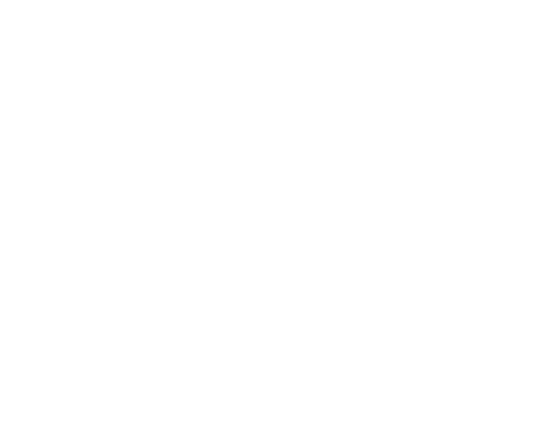
\includegraphics[width=4.5cm]{graphs/graph-dark-2}
        \endminipage
        \hfill\vrule width .4pt\hfill
        \minipage{.5\linewidth-1.2em}
        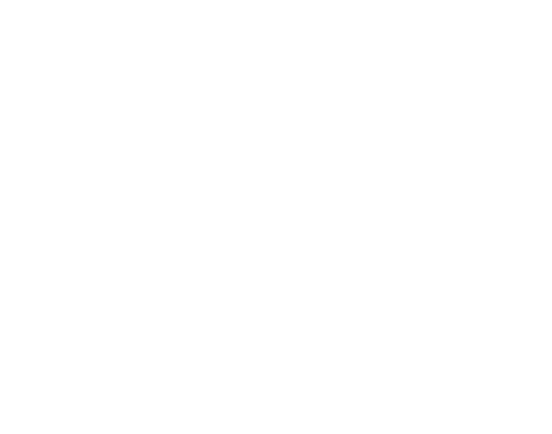
\includegraphics[width=4.5cm]{graphs/graph-dark-3}
        \endminipage
    \else 
        \begin{minipage}{.5\linewidth-1.2em}
        \centering
        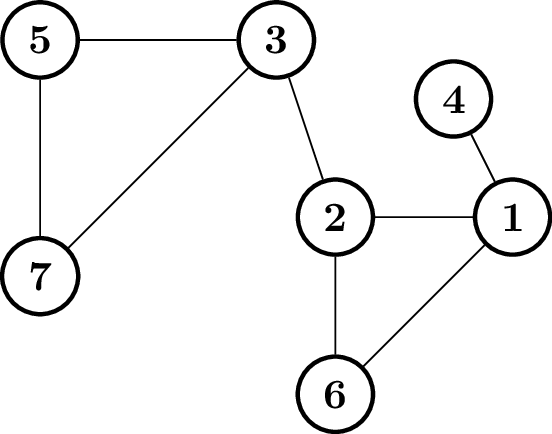
\includegraphics[width=4.5cm]{graphs/graph-2}
         \\ $(a)$ Une graphe $G$
        \end{minipage}
        \hfill\vrule width .4pt\hfill
        \begin{minipage}{.5\linewidth-1.2em}
            \centering
        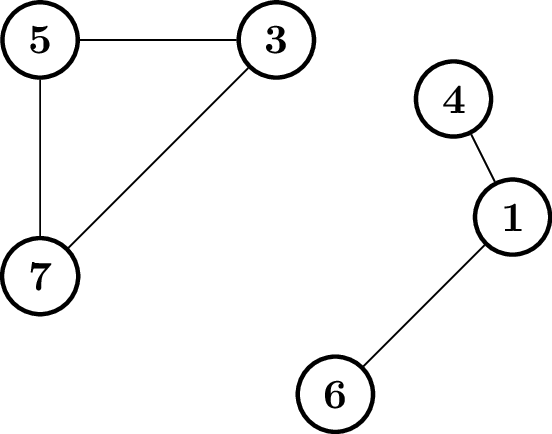
\includegraphics[width=4.5cm]{graphs/graph-3}
        \\ $(b)$ le graphe $G\backslash 2$
        \end{minipage}
    \fi 
    \captionof{figure}{Un graphe $G$ et le graphe $G\backslash 2$}
\end{center}


Soient $G_1=\left(S_1, A_1\right)$ et $G_2=\left(S_2, A_2\right)$ deux graphes non vides tels que $S_1$ et $S_2$ soient disjoints, c'est-à-dire tels que $S_1 \cap S_2=\varnothing$. Soit $s_1 \in S_1$ et soit $s_2 \in S_2$.
On définit le graphe $G=(S, A)$ avec $S=S_1 \cup S_2$ et $A=A_1 \cup A_2 \cup\left\{\left\{s_1, s_2\right\}\right\}$.


\xques\r %8
\<\lt{Montrer que :}
\Chi_G=\Chi_{G_1} \times \Chi_{G_2}-
\Chi_{G_1\backslash s_1 }  \times \Chi_{G_2 \backslash s_2}
 \>
\begin{solution}
    Notons $n_1$ et $n_2$ les cardinaux respectifs de $S_1$ et de $S_2$ et Soient $\sigma_1$ et $\sigma_2$ des indexations respectives de $S_1$ et de $S_2$ telles que $\sigma_1(1)=s_1$ et $\sigma_2(1)=s_2$. Considérons l'indexation $\sigma$ de $S=S_1\cup S_2$ définie par 
    \< 
        \sigma(k)=\xcases| 
            \sigma_1(k) & \text{si } k\in\iic{1,n_1} \\
            \sigma(k-n_1) & \text{si } k\in\iic{n_1+1,n_1+n_2}
        \.
    \>
    Par définition du graphe $G$ on a 
    \<
        M_{G,\sigma}=\xmatrix(
            M_{G_1,\sigma_1} & 
            E_{1,1} 
             \\
            \trans E_{1,1} & M_{G_2,\sigma_2}
        ) 
    \> 
    où $E_{1,1}$ est la première matrice de la base canonique de $\MN_{n_1,n_2}$. 
    Soit $\lambda\in\R$. Notons pour simplifier les écritures
    \< \al{}
        M_1(\lambda) &= \lambda I_{n_1}-M_{G_1,\sigma_1}=
            \delim\sz2(m_{i,j}^{(1)}(\lambda))_{i,j}  \\ 
        M_2(\lambda) &= \lambda I_{n_1}-M_{G_2,\sigma_2}=
        \delim\sz2(m_{i,j}^{(2)}(\lambda))_{i,j}
    \>
    \<\lt{Alors}
    \lambda I_{n_1+n_2}-M_{G,\sigma}=\begin{pmatrix}
            M_1(\lambda) &  K \\ \trans K & M_2(\lambda) 
        \end{pmatrix} 
        \quad\text{avec } 
        K=-E_{1,1} \in\MN_{n_1,n_2} 
    \>
    Soit un scalaire $\lambda$ qui ne soit pas une \vap de $M_{G_1,\sigma_1}$, de telle sorte que la matrice $M_1(\lambda)$ soit inversible. Nous pouvons alors écrire 
    \< 
        \xmatrix| I_{n_1} & 0 \\ -\trans KM_1(\lambda)^{-1} & I_{n_2} |\;
        \xmatrix| M_1(\lambda) &  K \\ \trans K & M_2(\lambda) | =
        \xmatrix| M_1(\lambda) & K \\ 0 & M_2(\lambda)-\trans KM_1(\lambda)^{-1}K|
    \>
    Le déterminant à gauche vaut $1$ donc nous avons 
    \<\n\lb{r&charinterm} \Chi_G(\lambda)= \xdet\sa2(M_1(\lambda))\xdet(M_2(\lambda)-\trans KM_1(\lambda)^{-1}K)\>
    Maintenant 
    \< 
        \trans K M_1(\lambda)^{-1}K=\trans E_{1,1}M_1(\lambda)^{-1}E_{1,1}=
        \xmatrix (\nu & 0 & \cdots & 0  \\
            0 &&& \vdots\\
            \vdots &&&\vdots \\
            0&\cdots&\cdots&0
        )\in\MN_{n_2}
    \>
    où $\nu$ est le coefficient d'indice $(1,1)$ de la matrice $M_1(\lambda)^{-1}$. Par linéarité du déterminant matriciel par rapport à chaque colonne nous avons donc
    \begingroup\def\arraystretch{1.4}
    \begin{align*}
    \xdet\sz2(M_2(\lambda)-\trans KM_1(\lambda)^{-1}K) &=
    {\xmatrix| 
    m_{1,1}^{(2)}(\lambda)-\nu & m_{1,2}^{(2)}(\lambda) & \cdots & m_{1,n_2}^{(2)}(\lambda) \\ 
    m_{2,1}^{(2)}(\lambda) &\cdots&\cdots& m_{2,n_2}^{(2)}(\lambda) \\
    \vdots &&& \vdots \\
    m_{n_2,1}^{(2)}(\lambda) &\cdots&\cdots& m_{n_2,n_2}^{(2)}(\lambda) |} 
    \\ &=
    \Chi_{G_2}(\lambda)-
    \nu{\xmatrix| 
    1 & m_{1,2}^{(2)}(\lambda) & \cdots & m_{1,n_2}^{(2)}(\lambda) \\ 
    0 &m_{2,2}^{(2)}(\lambda)&\cdots& m_{2,n_2}^{(2)}(\lambda) \\
    \vdots &\vdots&& \vdots \\
    0 &m_{n_2,2}^{(2)}(\lambda)&\cdots& m_{n_2,n_2}^{(2)}(\lambda) |} \\ &=
    \Chi_{G_2}(\lambda)-\nu\Chi_{G_2\backslash s_2}(\lambda)
    \end{align*}
    \endgroup
    L'expression de $\nu$ peut être prélevée dans la formule $A^{-1}=\textstyle(\xfrac1{{\det A}})\trans\com A$ valable pour toute matrice carrée inversible $A$:
    \<
        \nu=\frac{\Delta_{1,1}(M_1(\lambda))}{\det M_1(\lambda)}=
        \frac{\Delta_{1,1}(M_1(\lambda))}{\Chi_{G_1}(\lambda)}
    \>
    $\Delta_{1,1}(M_1(\lambda))$ est le déterminant de la matrice obtenue à partir de $M_1(\lambda)$ en éliminant la première ligne et la première colonne :
    \<
        \Delta_{1,1}(M_1(\lambda))=\Chi_{G_1\backslash s_1}(\lambda)
    \>
    \<\lt{soit au final}
        \nu=\frac{\Chi_{G_1\backslash s_1}(\lambda)}{\Chi_{G_1}(\lambda)}
    \>
    En revenant maintenant à l'\xeqref{charinterm} nous voyons que
    \<\fr{r}
        \Chi_G(\lambda)=\Chi_{G_1}(\lambda)\times \Chi_{G_2}(\lambda)-
        \Chi_{G_1\backslash s_1}(\lambda)\times \Chi_{G_2\backslash s_2}(\lambda)
    \>
    Égalité qui est valable pour tout $\lambda$ de l'ensemble infini $\R\setminus\mathrm{Sp}(M_{G_1,\sigma_1})$. Elle implique donc l'égalité des polynômes en jeu. 

\end{solution}

\xques %9
 Déterminer le polynôme caractéristique de la double étoile à $d_1+d_2+2$ sommets, constituée respectivement de deux étoiles disjointes à $d_1$ et $d_2$ branches, à qui l'on a ajouté une arête supplémentaire reliant les deux centres des deux étoiles.
Quel est le rang de la matrice d'adjacence de cette double étoile~?

\begin{solution}
    Soient $G_1$ et $G_2$ deux étoiles disjointes de sommets respectifs $s_1$ et $s_2$ et soit $G$ la réunion des deux graphes en ajoutant l'arête $\{s_1,s_2\}$. Selon la question précédente
    \<
    \Chi_G=\Chi_{G_1}\times \Chi_{G_2}-
        \Chi_{G_1\backslash s_1}\times \Chi_{G_2\backslash s_2}
    \>
    Ici les graphes $G_1\backslash s_1$ et $G_2\backslash s_2$ ont tous leurs sommets isolés (et donc leurs matrices d'adjacences sont nulles) donc $\Chi_{G_1\backslash s_1}=X^{d_1-1}$ et $\Chi_{G_2\backslash s_2}=X^{d_2-1}$. 
    Avec $\Chi_{G_1}=X^{d_1-2}(X^2-d_1)$ et $\Chi_{G_2}=X^{d_2-2}(X^2-d_2)$ on obtient
    \begin{xalign}
        \<
            \Chi_G &=
            X^{d_1+d_2-4}\delim\sa1(X^2-d_1)(X^2-d_2)-X^{d_1+d_2-2}
        \> 
        \eline 
        \<\lt{soit}\fr{r} 
            \sff &=
            X^{d_1+d_2-4}\delim\sz2(X^4-(d_1+d_2+1)X^2+d_1d_2)
        \>
    \end{xalign}
\end{solution}
\exit 

Dans toute la suite de ce problème, on suppose que $n$ est supérieur à 2 et on notera :
\xit\i+ N l'entier $\binom{n}{2}=\frac{n(n-1)}{2}$ 
\xit $\Omega_{n}$ l'ensemble des graphes de sommets $S=\iic{ 1, n }$
\xit $p_n$ un réel dépendant de $n$ appartenant à l'intervalle $\ii]0,1[$ et $q_n=1-p_n$.
\exit

Pour tous $i$ et $j$ appartenant à $S=\ii[[1, n]$ avec $i \neq j$, on note $X_{\{i, j\}}$ l'application de $\Omega_n$ dans $\{0,1\}$ telle que pour tout $G \in \Omega_n$ avec $G=(S, A)$ :
\<
    X_{\{i,j\}}(G)=\begin{cases} 
        1 & \text{si } \{i,j\} \in A \\
        0 &\text{si } \{i,j\} \notin A 
    \end{cases}
\>
Ainsi, $\left(X_{\{i, j\}}=1\right)=\left\{G \in \Omega_n \mid X_{\{i, j\}}(G)=1\right\}$ est l'ensemble des graphes de $\Omega_n$ dont $\{i, j\}$ est une arête. Réciproquement, on remarquera aussi que pour $G=(S, A)$, on peut écrire

\<
\{G\}=\xcap_{\{i, j\} \in A}\sa2(X_{\{i, j\}}=1)
 \xcap_{\{i, j\} \notin A}(X_{\{i, j\}}=0)
\>

On admet l'existence d'une probabilité $\Pr $ sur $\left(\Omega_n, \mathcal{P}\left(\Omega_n\right)\right)$ telle que les applications $X_{\{i, j\}}$ soient des variables aléatoires de Bernoulli de paramètre $p_n$ et indépendantes. On note $\mathcal{E}_n=\left(\Omega_n, \mathcal{P}\left(\Omega_n\right), \Pr \right)$ l'espace probabilisé ainsi construit.

Autrement dit, pour un graphe $G$ donné appartenant à $\Omega_n$, la probabilité qu'une arête $\{i, j\}$ soit contenue dans $G$ est $p_n$, et les arêtes apparaissent dans $G$ de façon indépendante.

\xques\r %10 
Soit $G=(S, A) \in \Omega_n$. Déterminer la probabilité $\Pr (\{G\})$ de l'événement élémentaire $\{G\}$ en fonction de $p_n, q_n, N$ et $a=\operatorname{card}(A)$.
Retrouver alors le fait que $\Pr \left(\Omega_n\right)=1$.

\begin{solution}
    Les événements $(\X{i,j}=1)$ et $(\X{i',j'}=0)$ avec $i,j,i',j'\in S$ sont tous mutuellement indépendants donc selon l'expression 
    \<\n\lb{eno1}
    \{G\}=\delim\sa4(\xcap_{\{i, j\} \in A}\sa2(X_{\{i, j\}}=1))
\bigcap \delim (\xcap_{\{i, j\} \notin A}(X_{\{i, j\}}=0))
    \> 
    \begin{nb} Attention ! Ne pas confondre $\{G\}$ et $G$.\end{nb}
    \begin{xalign}
        \<\lt{ona}
            \xPr\sz1(\{G\}) &=
            \xprod_{\{i,j\}\in A}\xPr\sa2(\X{i,j}=1)\times
            \xprod_{\{i,j\}\notin A}\xPr(\X{i,j}=0) 
        \> 
        \eline 
        \<\fr{r}\lt{soit}  \sff &=
            p_n^aq_n^{N-a}
        \>
    \end{xalign}
    le cardinal de $\OV A$ étant effectivement $N-a$ puisque $N=\ts\binom n2$ est le nombre de toutes les paires $\{i,j\}$ lorsque $i,j\in S$ et $i\ne j$. 

    Ensuite ; notons \emph{$\mathcal A$ l'ensemble de toutes les parties à deux éléments de $S$}. L'ensemble $\mathcal A$ est de cardinal $N$. Pour tout $a\in\iic{0,N}$, posons
    \<\Omega_{n,a}=\delim\sz2\{
        G=(S,A)\in\Omega_n \mid \card A=a\} 
    \>
    La famille $(\Omega_{n,a})_{a\in\iic{0,n}}$ est une partition de $\Omega_n$ donc
    \<\al{}
        \Pr(\Omega_n) &= 
        \sum_{a=0}^N\sum_{G\in\Omega_{n,a}}\Pr\delim\sz1(\{G\}) \\ &=
        \sum_{a=0}^N p_n^aq_n^{N-a}\card \Omega_{n,a}
    \>
    L'application $A\longmapsto G=(S,A)$ est une bijection de \score{3} l'ensemble $\mathcal P_a(\mathcal A)$ de toutes les parties de cardinal $a$ de $\mathcal A$ dans $\Omega_{n,a}$ donc 
    \< \card \Omega_{n,a}=\card\mathcal P_a(\mathcal A)=\binom Na\> 
    \<\lt{Ainsi}\fr{r}
        \Pr(\Omega)=\sum_{a=0}^N\binom Nap_n^a(1-p_n)^{N-a}=1
    \>
\end{solution}
\exit 

Dans la suite du problème on étudie la notion de fonction de seuil pour une propriété $\mathcal{P}_n$ vérifiée sur une partie des graphes de $\Omega_n$.

Une fonction de seuil pour la propriété $\mathcal{P}_n$ est une suite $\left(t_k\right)_{k \geq 2}$ de réels strictement positifs tels que :
\xit\i+ si $p_n=o\left(t_n\right)$ alors la limite, lorsque $n$ tend vers $+\infty$, de la probabilité pour que la propriété $\mathcal{P}_n$ soit réalisée vaut 0
\xit si $t_n=o\left(p_n\right)$ alors la limite, lorsque $n$ tend vers $+\infty$, de la probabilité pour que la propriété $\mathcal{P}_n$ soit réalisée vaut 1.
\exit

\wparti{Une première fonction de seuil}

\wpartii{Deux inégalités}
Soit $X$ une variable aléatoire définie sur un espace probabilisé $(\Omega, \mathcal{A}, \Pr )$ à valeurs dans $\N$ et admettant une espérance $\Es (X)$ et une variance $\Va (X)$.

\xques\r %11
\<\lt{Montrer que :} \Pr (X>0) \leq \Es (X) \>

 \begin{solution} 
    \<\lt{on a}\al{}
        \xEs(X) &= \sum_{n=0}^{+\infty} n\xPr(X=n) \\ &=
        \sum_{n=1}^{+\infty} n\xPr(X=n) \\ &\geq 
        \sum_{n=1}^{+\infty} \xPr(X=n) \\ &=
        \xPr(X>0)
    \>
    \<\lt{d'où}\fr{r} \xPr(X>0)\leq \xEs(X)\>
 \end{solution}

\xques %12
 Montrer que si $\Es (X) \neq 0$, alors $\Pr (X=0) \leq \frac{\Va (X)}{(\Es (X))^2}$.
 

\begin{ind} on remarquer que $(X=0) \subset\delim\sz1(|X-\Es (X)| \geq \Es (X))$.\end{ind}

\begin{solution}
    L'inclusion $(X=0) \subset(|X-\Es (X)| \geq \Es (X))$ fournie en indication est évidente puisque pour tout $\omega\in\Omega$
    \< X(\omega)=0\Lra |X(\omega)-\Es(X)|\geq |\Es(X)|=\Es(X) \>

    On en déduit que 
    $\xPr(X=0)\leq \xPr\sz1(|X-\Es(X)|\geq \Es(X))$ et ensuite selon l'inégalité de Bienaymé-Tchebychev 
    \<\fr{r}
        \Pr(X=0)\leq \frac{\Va(X)}{\Es(X)^2}
    \>
\end{solution}
\exit 

\wpartii{ Une fonction de seuil}

\xques\r %13
 Quelle est la loi suivie par la variable aléatoire $A_n$ représentant le nombre d'arêtes d'un graphe de $\Omega_n$ ?

 \begin{solution}
     La variable $A_n$ peut être écrite sous la forme
     \<
        A_n=\sum_{\{i,j\}\in\mathcal A}\X{i,j}
     \>
     où $\mathcal A$ désigne l'ensemble de toutes les paires de $\iic{1,n}$. Les variables $\X{i,j}$ sont mutuellement indépendantes et suivent toutes la loi de Bernoulli de paramètre $p_n$ et on a $\card \mathcal A=N$ donc
     \<\r
        La variable $A_n$ suit la loi binomiale de paramètres $(N,p_n)$ :
        $$ A_n\sim \mathscr B(N,p_n) $$
     \>
 \end{solution} 

\xques %14
 Montrer que si $p_n=o\left(\frac{1}{n^2}\right)$ au voisinage de $+\infty$, alors $\llim _{n \rightarrow+\infty} \Pr \left(A_n>0\right)=0$.
 \begin{solution}
    \<\lt{On a}\al{t}
         \Pr(A_n>0) &= 1-\Pr(A_n=0)=1-(1-p_n)^N 
         \\ &=
         1-\xexp(\frac{n(n-1)}2\ln(1-p_n)) \\ 
         \frac{n(n-1)}2\ln(1-p_n) & \sim-\frac12n^2p_n \qquad
         \makebox[0pt][l]{(avec $n^2p_n\longrightarrow 0$) }
     \>
     \<\r\lt{donc}
         si $p_n=\xpo(\frac1{n^2})$ alors $P(A_n>0) \longrightarrow 0$
     \>
  \end{solution}


\xques %15
 Montrer que si $\frac{1}{n^2}=o\left(p_n\right)$ au voisinage de $+\infty$, alors $\llim _{n \rightarrow+\infty} \Pr \left(A_n>0\right)=1$. 

 

\begin{solution}
    D'après la \poorref\n{Q12} on a  
    \<
        P(A_n)\leq \frac{\Va(A_n)}{\Es(A_n)^2}
    \>
    La variable $A_n$ suit la loi $\mathscr B(N,p_n)$ donc
    \<\al{} \Es(A_n)&=Np_n  &&& \Va(A_n)=Np_n(1-p_n) \>
    \<\lt{Alors}
        \frac{\Va(A_n)}{\Es(A_n)^2}=\frac{1-p_n}{Np_n}
        \leq \frac1{Np_n}
    \>
    Puisque $\ts\xfrac1{{n^2}}=\xpo(p_n)$ alors $n^2p_n\longrightarrow +\infty$ et donc $\ts\xfrac1{Np_n}\longrightarrow0$. On en déduit que $P(A_n)\lra0$ et ainsi 
    \<\r
         si $\frac1{n^2}=\xpo(p_n)$ alors $P(A_n>0) \longrightarrow 1$
     \>
\end{solution}

\xques%16
 En déduire une propriété $\mathcal{P}_n$ et sa fonction de seuil associée. 

 \begin{solution}
    \leavevmode 
    \<\r\wd{90}
        $P_n$ est la propriété :
        \<\t\wd{80}
            «le graphe aléatoire $G$ choisi selon le modèle du sujet possède au moins une arête» 
        \>
         sa fonction de seuil est la suite $(\ts\xfrac1{{n^2}})_{n\geq 2}$
    \>
 \end{solution}
\exit 

\wparti{Fonction de seuil de la copie d'un graphe}

Si $G=(S, A)$ est un graphe, on note $s_G$ (resp. $a_G$ ) le cardinal de $S$ (resp. $A$).

Soit $G_0=\left(S_0, A_0\right)$ un graphe particulier fixé. Par commodité d'écriture, on note $s_0=s_{G_0}$ le cardinal de $S_0, a_0=a_{G_0}$ le cardinal de $A_0$ et on suppose que $s_0 \geq 2$ et que $a_0 \geq 1$.


On va étudier la fonction de seuil de la propriété $\mathcal{P}_n$ : "contenir une copie de $G_0$ ".

On note $X_n^0$ la variable aléatoire réelle discrète définie sur l'espace probabilisé $\mathcal{E}_n$ telle que pour $G \in \Omega_n$, l'entier $X_n^0(G)$ est égal au nombre de copies de $G_0$ contenues dans $G$.

On introduit :
\xit\i+ l'ensemble $\mathcal{C}_0$ des copies de $G_0$ dont les sommets sont inclus dans $\iic{ 1, n }$ :
\<
\mathcal{C}_0=\delim\sz2\{H \mid H \text { est une copie de } G_0 \text { et } H=\left(S_H, A_H\right) \text { avec } S_H \subset \iic{ 1, n }\}
\>
\xit  pour un graphe $H=\left(S_H, A_H\right)$ avec $S_H \subset\ii[[1, n]$, la variable aléatoire suivant une loi de Bernoulli $X_H$ définie par :
\<
\forall G \in \Omega_n \quad X_H(G)= \begin{cases}1 & \text { si } H \subset G \\ 0 & \text { sinon }\end{cases}
\>
\xit  le réel $\omega_0$ défini par :
\<
\omega_0=\min _{\substack{H \subset G_0 \\ a_H \geq 1}} \frac{s_H}{a_H}
\>
\exit 

\xques\r %17
 \<\lt{Montrer que}
\Es \left(X_H\right)=p_n^{a_H} .
\>

\begin{solution}
    %Sachant que $S_H\subset \iic{1,n}$, considérons le graphe 
    %$H'=(\iic{1,n},A_H)$ dont l'ensemble des sommets est $\iic{1,n}$. Puisque par définition $A_{H'}=A_H$ alors $H\subset G$ si et seulement si $H'\subset G$. 
    Sachant que $S_H\subset \iic{1,n}$ on a pour tout $G\in\Omega_n$
    \< H\subset G\Llra A_H\subset A_G\> 
    \<\lt{donc}
        (X_H=1)=\delim\sz2\{
            G\in\Omega_n\mid A_H\subset A_G 
        \}
    \>
    On peut donc créer une partition de $(X_H=1)$ sous la forme
    \<
        (X_H=1)=\xcup_{b=0}^{N-a_H}\delim\sz2\{
            G\in\Omega_n\mid A_H\subset A_G\text{ et } a_G=a_H+b
        \}
    \>
    Or pout tout $b\in\iic{1,N-a_H}$, il y a $\ts\binom{N-a_h}{b}$ façon de compléter $A_H$ en une partie de $\mathcal A$ de cardinal $a_H+b$ et pour chaque partie $A$ de $\mathcal A$ qui vérifie cette condition on a selon la \poorref{Q10}  
    \< \xPr\sz1(\{(S,A)\})= p_n^{a_H+b}q_n^{N-a_H-b} \>
    \<\lt{donc}\compactbreak{
        \xPr(
            \delim\sz2\{
            G\in\Omega_n\mid A_H\subset A_G\text{ et } a_G=a_H+b
        \}
        )= {} \ifcompact\qquad\fi \\
         \binom{N-a_h}b p_n^{a_H+b}q_n^{N-a_H-b}
    }
    \>
    \<\lt{par suite}\al{}
        \Pr(X_H=1) &=
        p_n^{a_H}\sum_{b=0}^{N-a_H}\binom{N-a_h}b p_n^{b}(1-p_n)^{N-a_H-b}=p_n^{a_H}
    \>
    La variable $X_H$ suit une loi de Bernoulli donc 
    \<\fr{r}
        \Es(X_H)=\Pr(X_H=1)=p_n^{a_H}
    \>
\end{solution}

\xques %18
 Soit $S_0^{\prime}$ un ensemble fixé de cardinal $s_0$. On note $c_0$ le nombre des graphes dont l'ensemble des sommets est $S_0^{\prime}$ et qui sont des copies de $G_0$.

Exprimer le cardinal de $\mathcal{C}_0$ à l'aide de $c_0$ et en utilisant un majorant simple de $c_0$, justifier que le cardinal de $\mathcal{C}_0$ est inférieur à $n^{s_0}$.

\begin{solution}
    Récapitulons les notations :
    \begin{xitem}
        \xit Au départ il y a le graphe $G_0=(S_0,A_0)$ avec $s_0=\card S_0\geq 2$ et $a_0=\card A_0\geq 1$ ;
        \xit $\mathcal C_0$ est l'ensemble des graphes dont les sommets sont contenus dans $\iic{1,n}$ et qui sont des copies de $G_0$ (on notera que forcément $s_0\leq n$);
        \xit $S_0'$ est un (autre) ensemble de sommets de même cardinal $s_0$ que $S_0$ et $c_0$ est le nombre de graphes de sommets $S_0'$ et qui sont des copies de $G_0$. 
    \end{xitem} 
    Notons $C'_0$ l'ensemble des graphes de sommets $S_0'$ qui sont des copies de $G_0$. Soit $S$ une partie quelconque de $\iic{1,n}$ de cardinal $s_0$ et fixons une bijection $\sigma:S\longmapsto S'_0$. Définissons ensuite pour tout graphe $(S,A)$ de sommets $S$ le graphe $(S_0',A_\sigma)$ de sommets $S_0'$ par 
    \< A_\sigma=\delim\sz2\{
        \{\sigma(i),\sigma(j)\}\mid \{i,j\}\in A
        \} 
    \>
    L'application $(S,A)\longmapsto (S'_0,A_\sigma)$ ainsi construite est une bijection. 
    Le graphe $(S,A)$ est une copie de $G_0$ si et seulement si $(S'_0,A_\sigma)$ en est une. Il y a donc une bijection entre $\mathcal C_0'$  et l'ensemble des graphes de sommets $S$ qui sont des copies de $G_0$. Maintenant, si on note $C(S)$ l'ensemble des graphes de sommets $S$ qui sont des copies de $G_0$ alors on vient de justifier que $|C(S)|=c_0$. Grâce à la partition :
    \<
        \mathcal C_0=\xcup_{S\in\mathcal P_{s_0}(\iic{1,n})} C(S)
    \> 
    \<\r\lt{on conclut que}
        $|\mathcal C_0|=\binom n{s_0}c_0$
    \>
    Fixons maintenant un graphe $(S'_0,B_0)$ dans $C'_0$ et posons pour toute permutation $\rho$ de $S'_0$ 
    \< 
        B_\rho=\delim\sz2\{
            \{\rho(i),\rho(j)\}\mid \{i,j\}\in B_0
        \}
    \>
    Par définition mème des copies d'un graphe, pour tout élément $(S'_0,B)$ de $C'_0$ il existe $\rho$ telle que $B=B_\rho$, indiquant que l'application 
    $\rho\longmapsto (S'_0,B_\rho)$ est une surjection de l'ensemble des permutations de $S'_0$ dans $C'_0$. On en déduit que 
    \< c_0\leq s_0! \> 
    \<\lt{Par suite}\fr{r}
        |\mathcal C_0|=\frac{n(n-1)\cdots(n-s_0+1)}{s_0!}c_0\leq n^{s_0}
    \>
\end{solution}

\xques %19
 Exprimer $X_n^0$ à l'aide de variables aléatoires  du type $X_H$, et montrer que :
 \<
\Es \left(X_n^0\right)=\sum_{H \in \mathcal{C}_0} \Pr (H \subset G) \leq n^{s_0} p_n^{a_0} .
\>

\begin{solution}
    Rappelons, pour tout graphe $G\in\Omega_n$, les notations 
    \begin{xitem}
        \xit $X_H(G)$ vaut $1$ si $H\subset G$, $0$ sinon ;
        \xit $X_n^0(G)$ est le nombre de copies de $G_0$ contenues dans $G$ ;
        \xit $\mathcal C_0$ est l'ensemble de toutes les copies de $G_0$ dont les sommets sont dans $\iic{1,n}$. 
    \end{xitem}
    \<\r\lt{Visiblement}
          $X_n^0=\sum_{H\in \mathcal C_0} X_H$
    \>
    On en déduit par linéarité de l'espérance que 
    \<\al{}
        \Es(X_n^0) &= \sum_{H\in \mathcal C_0}\Es(X_H) 
        \\ &=
        \sum_{H\in \mathcal C_0}p_n^{a_H} 
        \\ &=
        \sum_{H\in \mathcal C_0}p_n^{a_0}
        \\ &=
        p_n^{a_0}|\mathcal C_0|
    \>
    \<\fr{r}\lt{et donc}
          \Es(X_n^0)\leq n^{s_0}p_n^{a_0}
    \>
\end{solution}

\xques %20
 En déduire que si $p_n=o\left(n^{-\omega_0}\right)$, alors $\llim _{n \rightarrow+\infty} \Pr \left(X_n^0>0\right)=0$.

\begin{ind} on pourra introduire $H_0 \subset G_0$ réalisant le minimum donnant $\omega_0$.
\end{ind}

\begin{solution}
    Soit $H_0$ un sous graphe de $G_0$ tel que 
    \< \omega_0=\xfrac{s_{H_0}}{a_{H_0}} \> 

    On définit la variable $Y_0^n$ liée à $H_0$ de la même façon que $X_0^n$ est liée à $G_0$. 
    Puisque $H_0\subset G_0$, tout graphe $G$ de $\Omega_n$ contient au moins autant de copies de $H_0$ que de copies de $G_0$. C'est à dire que $X_0^n\leq Y_0^n$ et par croissance de l'espérance on a donc
    \< \Es(X_n^0)\leq \Es(Y_n^0) \>
    D'après la question précédente on a donc 
    \<\n\lb{m&x0nmaj}
         0\leq \Es (X_n^0)\leq n^{s_{H_0}}p_n^{a_{H_0}}
    \>
    Or par hypothèse $p_n=\xpo(n^{-\omega_0})$ donc
    \< 
        n^{s_{H_0}}p_n^{a_{H_0}} =
        \xpo\sz2(n^{s_{H_0}-\omega_0 a_{H_0}})=\osymb(1) 
    \>
    D'après la \xeqref{x0nmaj} on a donc $\Es(X_0^n)\longrightarrow 0$. D'autre part, comme dans la \poorref{Q14}
    \<\al{}
        \Pr(X_n^0>0) &=\sum_{k=1}^{+\infty}\Pr(X_n^0=k)
        \\ &\leq 
        \sum_{k=1}^{+\infty} k\Pr(X_n^0=k) 
        \\ &\leq 
        \Es(X_n^0)
    \>
    \<\fr{r}\lt{at ainsi}
          \lim \Pr(X_n^0>0)=0
    \>
\end{solution}
\exit

On suppose dorénavant que $\llim _{n \rightarrow+\infty}\left(n^{\omega_0} p_n\right)=+\infty$.

\xques\r %21
Montrer que l'espérance $\xEs\sz2(\delim\sz1(X_n^0)^2)$ vérifie :
\<
\xEs\sz2(\delim\sz1(X_n^0)^2)=\sum_{\left(H, H^{\prime}\right) \in \mathcal C_0^2} \Pr \left(H \cup H^{\prime} \subset G\right)=\sum_{\left(H, H^{\prime}\right) \in \mathcal C_0^2} p_n^{2 a_0-a_{H \cap H^{\prime}} .} .
\>
\begin{mini}{errata}
    Cette formule est ambiguë puisqu'elle ne précise pas la nature du $G$ dans \og l'événement\fg $(H\cup H'\subset G)$, ni celle des «graphes»  $H\cup H'$ et $H\cap H'$. Le développement dans le corrigé les introduira de façon naturelle. 
\end{mini}

\begin{solution} Rappelons l'expression 
    \<
        X_n^0=\sum_{H\in \mathcal C_0}X_H 
    \>  
    \<\lt{donc}
        \delim\sz2(X_n^0)^2=\sum_{H,H'\in \mathcal C_0}X_H X_{H'}
    \>
    \<\lt{et par linéarité de l'espérance}
        \xEs\sz2((X_n^0)^2) =
        \sum_{H,H'\in \mathcal C_0}E(X_HX_{H'})
    \>
    Notons pour deux graphes $H=(S,A), H'=(S',A')$, 
    \<\al{}
        HUH' &= (S\cup S',A_H\cup A_{H'}) \\
        H\cap H' &=(S\cup S',A_H\cap A_{H'})
    \>
     On remarquera dès lors que si $G$ est un graphe de $\Omega_n$ alors
    \<\al{}
        H\cup H'\subset G &\Llra 
        S_{H}\cup S_{H'}\subset S_{G}\text{ et }A_{H}\cup A_{H'}\subset A_{G} \\ &\Llra 
        S_H\subset S_G \text{ et } A_H\subset A_G\text{ et }
        S_{H'}\subset S_G \text{ et } A_{H'}\subset A_G
        \\ &\Llra
        H\subset G\text{ et } H'\subset G
    \>
    \<\lt{et que}\al{}
        a_{H\cup H'} &= 
        |A_{H}\cup A_{H'}| \\ &=
        |A_H|+|A_{H'}|-|A_{H}\cap A_{H'}| \\ &=
        a_{H}+a_{H'}-a_{H\cap H'}
    \>
    Soient maintenant $H,H'\in \mathcal C_0$. Alors la variable $X_HX_{H'}$ ne peut prendre que les valeurs $0$ et $1$, c'est à dire qu'elle suit une loi de Bernoulli.  
    \<\lt{De plus}\al{} 
        (X_HX_{H'}=1) &= 
        (X_H=1)\cap(X_{H'}=1)  \\ &=
        \delim\{ G\in\Omega_n\mid H\subset G \}\cap 
        \delim\{ G\in\Omega_n\mid H'\subset G \} \\ &=
        \boxed{\delim\{ G\in\Omega_n\mid H\cup H'\subset G \}} \\ &=
        (X_{H\cup H'}=1)
        \>
    \<\lt{et donc}\fr{}
        \Pr(X_HX_{H'}=1)=\Pr(X_{H\cup H'}=1)=p_n^{2a_0-a_{H\cap H'}}\>
    \begin{nb}
        $X_HX_{H'}$ et $X_{H\cup H'}$ étant des variables de Bernoulli, l'égalité  $(X_HX_{H'}=1)=(X_{H\cup H'}=1)$ signifie en fait que 
        \<\n\fr{}\lb{hcuphprime}    
             X_HX_{H'}=X_{H\cup H'} 
        \>
        \<\lt{et la relation}
            (X_n^0)^2=
            \sum_{H,H'\in\mathcal C_0} X_{H\cup H'}
        \>
        confirme le fait que $(X_n^0)^2(G)$  est le nombre de double-copies de $G_0$ contenues dans le graphe $G$ (y compris les double-copies de la forme $H\cup H$).
    \end{nb}
    \begin{nb}
        Finalement le curieux événement $(H\cup H'\subset G)$ pouvait être écrit de façon plus compréhensible sous la forme 
        \< \delim\{ G\in\Omega_n\mid H\cup H'\subset G \} \>
        \<\lt{ou encore mieux}
            (X_HX_{H'}=1)
        \>
   \end{nb}

    $X_HX_{H'}$ est donc la variable de Bernoulli $X_{H\cup H'}$ de paramètre 
    \< 
        \Pr(X_{H\cup H'}=1)=
        \Es(X_{H\cup H'})=p_n^{a_{H\cup H'}}=
        p_n^{2a_0-a_{H\cap H'}}
    \>
    \<\r\lt{finalement}
        $\xEs\sz2((X_n^0)^2)=\sum_{H,H'\in \mathcal C_0}p_n^{2a_0-a_{H\cap H'}}$
    \>
\end{solution}
\exit 

Pour $k \in\left[0, s_0\right]$, on note :
\<
\Sigma_k=\sum_{\substack{\left(H, H^{\prime}\right) \in \mathcal C_0^2 \\ s_{H \cap H^{\prime}}=k}} \Pr \left(H \cup H^{\prime} \subset G\right) .
\>

\xques\r %22
\<\lt{Montrer que :} 
    \Sigma_0 \leq\left(\Es \left(X_n^0\right)\right)^2
\>

 \begin{solution}
    On a par définition (après adaptation des notations)
    \<\n\lb{sigma0leq}
    \Sigma_0=\xsum\ss{cs,cl}_{\left(H, H^{\prime}\right) \in \mathcal C_0^2 \\ S_{H} \cap S_{H^{\prime}}=\varnothing}\xPr\sz2(\{G\in\Omega_n\mid H \cup H^{\prime} \subset G\})=
    \xsum\ss{cs,cl}_{\left(H, H^{\prime}\right) \in \mathcal C_0^2 \\ S_{H} \cap S_{H^{\prime}}=\varnothing} 
    \xEs\sz1(X_{H\cup H'})
    \>
    \<\lt{donc}
    \Sigma_0 =\xsum\ss{cs,cl}_{\left(H, H^{\prime}\right) \in \mathcal C_0^2 \\ S_{H} \cap S_{H^{\prime}}=\varnothing} p_n^{2a_0-a_{H\cap H'}}
    \>
    Or si $S_H\cap S_{H'}=\varnothing$ alors $A_{H}\cap A_{H'}=\varnothing$ et donc $a_{H\cap H'}=0$. Ainsi
    \<
          \Sigma_0=\delim\sz3|\delim\sz2\{(H,H')\in (\mathcal C_0)^2\mid S_H\cap S_H'=\varnothing\}| p_n^{2a_0}\leq
          |(\mathcal C_0)^2|p_n^{2a_0}=\xEs\sz1(X_n^0)^2
    \>
    \<\fr{r}
        \Sigma_0 \leq \xEs\sz1(X_n^0)^2
    \>
    \begin{mini}{Autre méthode}
        On peut procéder autrement en remarquant que pour tout $G\in\Omega_n$
        \< 
            X_H(G)=1 \Llra 
            \xforall \{i,j\}\in A_H\; \X{i,j}(G)=1
        \>
        \<\lt{ce qui signifie que}
              X_H=\prod_{\{i,j\}\in A_H}\X{i,j}
        \>
        Si maintenant $S_H\cap S_{H'}=\varnothing$ alors $A_H\cap A_{H'}=\varnothing$. Les variables $\X{i,j}$ sont mutuellement indépendantes  donc par lemme des coalitions les variables $X_H$ et $X_{H'}$ sont indépendantes. En particulier $E(X_HX_{H'})=E(X_H)E(H')$. En reprenant à l'étape 
        \xeqref{sigma0leq} 
        \<\al{} 
            \Sigma_0 &= 
            \xsum\ss{cs}_{\left(H, H^{\prime}\right) \in \mathcal C_0^2 \\ S_{H} \cap S_{H^{\prime}}=\varnothing} 
            \Es(X_{H})\Es(X_{H'}) 
            \\ &\leq
            \xsum_{\left(H, H^{\prime}\right) \in \mathcal C_0^2}\Es(X_{H})\Es(X_{H'}) 
            \\ &=
            \delim\sz3(\sum_{H\in C_0}E(X_H))^2 
            \\ &=
            \delim\sz1(\Es(X_n^0))^2
    \>
    \end{mini}
 \end{solution}

\xques %23
 Soit $k \in \iic{ 1, s_0 } ;$ montrer que :
\<
\Sigma_k \leq \sum_{H \in \mathcal{C}_0}\binom{s_0}{k}\binom{n-s_0}{s_0-k} c_0 p_n^{2 a_0} p_n^{-\frac{k}{\omega_0}} .
\>

\begin{solution}
    D'après les questions précédentes on a 
    \<
        \Sigma_{k} =
        \xsum\ss{cs}_{H,H'\in \mathcal C_0\\ s_{H\cap H'}=k}
        p_{n}^{2a_0-a_{H\cap H'}} 
    \>
    qu'on peut réécrire sous la forme
    \<
        \Sigma_{k} =
        \sum_{H\in\mathcal C_0}
        \xsum\ss{cs}_{H'\in\mathcal C_0 \\ s_{H\cap H'}=k}
        p_{n}^{2a_0-a_{H\cap H'}}
    \>
    Fixons maintenant un graphe $H\in\mathcal C_0$ et considérons l'ensemble
    \< 
        \Omega_{H}=\ens\sz2{(S,A)\in\mathcal C_0\tq1 |S\cap S_H|=k}
    \>
    Considérons ensuite l'application 
    \<
        \func{}
            {\Omega_H}
            {\mathcal P_{k}(S_H)\times \mathcal P_{s_0-k}(\iic{1,n}\setminus S_H)}
            {(S,A)}
            {\delim\sz1(S\cap S_H, S\setminus (S\cap S_H))}
    \>
     Cette application est surjective car pour tout couple $(S_1,S_2)\in \mathcal P_{k}(S_H)\times \mathcal P_{s_0-k}(\iic{1,n}\setminus S_H)$ il y a au moins une copie du graphe $G_0$ de sommets $S=S_1\cup S_2$ (moyennant une bijection $\sigma:S_0\longrightarrow S$) et que $|S\cap S_H|=|S_1|=k$. Ensuite toute copie de $G_0$ de sommets $S=S_1\cup S_2$ et un élément de $\Omega_H$. Or d'après la \poorref{Q18}, le nombre de ces copies est $c_0$. Donc tout élément de $\mathcal P_{k}(S_H)\times \mathcal P_{s_0-k}(\iic{1,n}\setminus S_H)$ admet exactement $c_0$ antécédents par notre application. Alors
     \< 
        |\Omega_H|=c_0\delim\sz1|\mathcal P_{k}(S_H)\times \mathcal P_{s_0-k}(\iic{1,n}\setminus S_H)|=c_0\binom{s_0}k\binom{n-s_0}{s_0-k}
     \>
    Par définition du nombre $\omega_0$ on a 
    \< 
        \xforall H'\in\Omega_H\; a_{H\cap H'}\leq 
        \frac{s_{H\cap H'}}{\omega_0}=\frac k{\omega_0}
    \>
    Puisque $p_n\in\ii]0,1[$ on a donc
    \< 
        \xforall H'\in\Omega_H\; 
        p_n^{-a_{H\cap H'}}\leq 
        p_n^{-\frac k{\omega_0}}
    \>
    Ce qui achève de justifier que
    \<\fr{r}
        \Sigma_k\leq 
        \sum_{H\in\mathcal C_0}
        c_0\binom{s_0}k\binom{n-s_0}{s_0-k}
        p_{n}^{2a_0-\frac{k}{\omega_0}}
    \> 
    Noter que $k$ et $n$ ne dépendent pas de l'indice $H\in\mathcal C_0$ donc en fait 
    \<\fr{r}
        \Sigma_k\leq 
        |C_0|c_0\binom{s_0}k\binom{n-s_0}{s_0-k}
        p_{n}^{2a_0-\frac{k}{\omega_0}}
    \>
\end{solution}

\xques %24
 Justifier que pour tous entiers naturels $q$ et $r$ vérifiant $1 \leq q \leq r$, on a :
 \<
\binom{r}{q} r^{-q} \geq \frac{1}{q!}\left(1-\frac{q-1}{q}\right)^q
\>
et en déduire que pour $k \in\left[1, s_0\right]$, on a 
$\Sigma_k=\xpo\sz2(\Es(X_n^0)^2)$ lorsque $n$ tend vers $+\infty$.

\begin{solution}
    \<\al{}
        \binom rq r^{-q} &=
        \frac{r(r-1)\cdots(r-q+1)}{q!} r^{-q} 
        \\ &=
        \frac1{q!}\cdot1\cdot
        \delim(1-\frac 1r)
        \delim(1-\frac2r)\cdots\delim(1-\frac{q-1}r) 
        \\ &\geq 
        \frac1{q!}\delim(1-\frac{q-1}q)^{q}
    \>
    Rappelons que 
    $\Es(X_n^0)= p_n^{a_0}|\mathcal C_0|$ et $|\mathcal C_0|=\ts\binom n{s_0}c_0$. On a 
    \< \al{}
        \frac{\Sigma_k}{\Es(X_n^0)^2} &\leq
        \frac1{\Es(X_n^0)^2}c_0|\mathcal C_0| \binom{s_0}k\binom{n-s_0}{s_0-k}
        p_{n}^{2a_0-\frac{k}{\omega_0}}
        \\ &\leq
        \frac{c_0}{|\mathcal C_0|}
        \binom{s_0}k\binom{n-s_0}{s_0-k}
        p_{n}^{-\frac{k}{\omega_0}}
        \\ &\leq 
        \frac{1}{\binom n{s_0}}
        \binom{s_0}k\binom{n-s_0}{s_0-k}
        p_{n}^{-\frac{k}{\omega_0}}
    \>
    Maintenant $\binom n{s_0}=\frac{n(n-1)\cdots(n-s_0+1)}{s_0!}\geq \frac1{s_0!}(n-s_0)^{s_0}$ donc en posant $M=s_0!\binom{s_0}k$ on a 
    \< \al{}
        \frac{\Sigma_k}{\Es(X_n^0)^2} 
        &\leq 
        M\binom{n-s_0}{s_0-k}(n-s_0)^{-s_0}p_{n}^{-\frac{k}{\omega_0}}
        \\ &\leq 
        M\binom{n-s_0}{s_0-k}(n-s_0)^{k-s_0}(n-s_0)^{-k}p_{n}^{-\frac{k}{\omega_0}}
        \\ &\leq 
        \frac M{(s_0-k)!}\delim(1-\frac{s_0-k-1}{s_0-k})^{s_0-k}
        (n-s_0)^{-k}p_{n}^{-\frac{k}{\omega_0}}
    \>
    et vu que $(n-s_0)^{-k}\sim n^{-k}$ il existe une constante $M'>0$ telle que $(n-s_0)^{-k}\leq M'n^{-k}$ pour tout $n\in\N^*$. On a lors  
    \< 
    0\leq\frac{\Sigma_k}{\Es(X_n^0)^2} \leq M'' n^{-k}p_n^{-\frac{k}{\omega_0}}=M''\delim\sz1(n^{\omega_0}p_n)^{-k/\omega_0}
    \>
    où $M''=\frac {MM'}{(s_0-k)!}\delim(1-\frac{s_0-k-1}{s_0-k})^{s_0-k}$.
    Puisque $n^{\omega_0}p_n\lra0$ cela implique que 
    \<\fr{r} \Sigma_k=\xpo\sz1(\Es(X_n^0)^2)\>
\end{solution}

\xques %25
\<\lt{Montrer que :} \llim _{n \rightarrow+\infty} \frac{\Va\left(X_n^0\right)}{\left(\Es \left(X_n^0\right)\right)^2}=0. \> %où $\Va \left(X_n^0\right)$ désigne la variance de $X_n^0$.

 \begin{solution}
    En partitionnant l'ensemble $\mathcal C_0^2$ sous la forme 
    \< \mathcal C_0^2=
        \xcup_{k=0}^{s_0}\sz3\{(H,H')\in\mathcal C_0^2\tq1
        s_{H\cap H'}=k\} boh
    \> 
    les formules de la \poorref\n{Q21} signifient que 
    \<\xEs\sz1((X_n^0)^2)=\sum_{k=0}^{s_0}\Sigma_k\>
    \<\lt{et donc}
        \frac{\xVa\sz1(X_n^0)}{\xEs\sz1(X_n^0)^2}=
        \frac{\Sigma_0}{\xEs\sz1(X_n^0)^2}-1+\sum_{k=1}^{s_0}\frac{\Sigma_k}{\xEs\sz1(X_n^0)^2}
    \>
    \<\lt{Il s'agit donc de montrer que} 
        \frac{\Sigma_0}{\xEs\sz1(X_n^0)^2}\longrightarrow 1
    \>
    \<\lt{Or}
        \Sigma_0=\xEs\sz3(\xsum\ss{cs}_{H,H'\in\mathcal C_0 \\ S_H\cap S_{H'}=\varnothing}X_{H}X_{H'})=
        \xEs\sz4(\xsum_{H\in\mathcal C_0}X_H\delim\sz3(\underset{Y_H}{\underbrace{\xsum\ss{cs}_{H'\in\mathcal C_0 \\ S_{H'}\subset \iic{1,n}\setminus S_H}X_{H'}}}))
    \>
    Par lemme des coalitions la variable $Y_H$ est indépendante de $X_H$ car toutes les variables $X_{H'}$ sont indépendantes de $X_H$. De plus elle suit la même loi que $X_{n-s_0}^0$. Donc 
    \< \al{}
        \Sigma_0 &=
        \sum_{H\in\mathcal C_0}\Es(X_H)\Es(Y_H) 
        \\ &=
        \sum_{H\in\mathcal C_0}\Es(X_H)\Es(X_{n-s_0}^0) 
        \\ &= 
        \Es(X_{n}^0)\Es(X_{n-s_0}^0) 
    \>
    Des calculs effectués précédemment dans les questions \poorref\n\c{Q18} et \poorref\n\c{Q19} donnent 
    \< 
        \Es(X_n^0)=|C_0|p_n^{a_0}=c_0\binom{n}{s_0}p_n^{a_0} 
    \>
    $c_0$ étant une constante indépendante de $n$ on a donc
    \< 
        \Es(X_{n-s_0}^0)=c_0\binom{n-s_0}{s_0}p_n^{a_0}
        \sim c_0\binom{n}{s_0}p_n^{a_0} =
        \Es(X_n^0)
    \>
    \<\lt{et ainsi } \Sigma_0\sim \delim\sz1(E(X_n^0))^2 \>
    Ce qui achève la démonstration.
    \<\fr{r} 
    \lim _{n \to +\infty} \frac{\Va(X_n^0)}{\xEs\sz1(X_n^0)^2}=0
    \>
 \end{solution}

\xques %26 
 Montrer alors que la suite $\left(k^{-\omega_0}\right)_{k \geq 2}$ est une fonction de seuil pour la propriété $\mathcal{P}_n$.
 \begin{solution}
    Découle des questions \poorref\n{Q12}, \poorref\n{Q20} et \poorref\n{Q25}
 \end{solution} 

\xques %27 \triangleright$ 
Retrouver le résultat de la \poorref{Q16} 
et déterminer une fonction de seuil pour la propriété « contenir une copie de l'étoile à $d$ branches" avec $d$ entier fixé supérieur à 1.

 \begin{solution}
    La variable $A_n$ est en fait égale à $X_n^0$ lorsque le graphe $G_0$ est formé de deux sommets et une arête. Dans ca cas le seul graphe $H\subset G_0$ qui contient au moins une arête est $G_0$ lui même et par suite 
    \<\fr{r} \omega_0=2\> 
    On retrouve ainsi le résultat de la \poorref{Q16}.

    Lorsque $G_0$ est une étoile à $d\geq 1$ branches alors un sous graphe $H\subset G_0$ est soit a sommets isolés s'il ne contient pas le centre $s$ de $G_0$, soit il est lui même une étoile s'il le contient. Donc 
    \< \omega_0=\min_{2\leq k\leq d}\frac{k}{k-1} \>
    Comme  pour tout $k\in\iic{2,d}$, 
    \<
        \frac{k}{k-1}-\frac{d}{d-1}=\frac{k(d-1)-d(k-1)}{(k-1)(d-1)}=\frac{d-k}{(k-1)(d-1)}\geq0
    \>
    \<\fr{r}\lt{alors} \omega_0=\frac{d}{d-1} \> 
 \end{solution}

 \exit

 \vskip 0pt plus .25fill
 \centering 
 {\scshape Fin du problème}
 \vfill

\end{enonce} 

\solutions

\end{document}